\documentclass{beamer}
\usepackage{tikz}
\usetikzlibrary{trees,arrows}

\usetheme{CMU}

\title{AutoMerge}
\subtitle{}
\date{\today}
\author[Fonseca Mesner]{Francisco Fonseca \and Octavio Mesner}
\institute{Carnegie Mellon University}

\begin{document}
\maketitle

\section{}
\begin{frame}
\frametitle{Goals}
Discuss
\begin{itemize}
\item Outline Problem
\item Alternatives
\item Explain Costs and Calculations
\item Specify Uncertainty
\item State Assumptions
\item Show Results
\item Convey Sensitivity Analyses
\item Conclusion
\end{itemize}
\end{frame}

\section{Problem}

\begin{frame}
  \frametitle{Problem}
  \framesubtitle{Overview}
  \begin{itemize}
  \item NYC to become a leader in \emph{smart city} infrastructure
  \item One piece: Evaluate autononous vehicles
  \item By 2020, NYC expects its fleet to be autonomous.
  \item We will evaluate AutoMerge (AM) Inc as an alternative.
  \end{itemize}
\end{frame}

\section{Alternatives}
\begin{frame}
  \frametitle{Alternatives}
  \begin{enumerate}
  \item Do not not implement AM
  \item Implement AM
  \item Perform a pilot study
  \end{enumerate}
\end{frame}

\begin{frame}
  \frametitle{Missing Data}
  \centering
  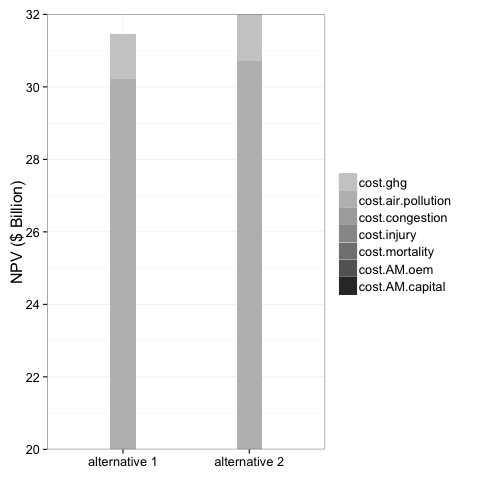
\includegraphics[width=0.75\textwidth]{../../R/barplot1}
\end{frame}

\section{Methods}

\subsection{Evaluation}
\begin{frame}
  \frametitle{Cross Validation}
  How well does a model perform on new data?
  \centering
  %\includegraphics[width=0.9\textwidth]{10foldCv}
\end{frame}

\subsection{Lasso}
\begin{frame}
  \frametitle{What is Lasso?}
  \begin{itemize}
    \item Builds on multiple linear regression
    \item Includes a penalty term for size of parameters
  \end{itemize}
  \centering
  %\includegraphics[width=0.6\textwidth]{lassoPlot}
\end{frame}

\end{document}
